\section{Elektroplanung und Realisierung \textcolor{gray}{(Nikolaj Voglauer)}}

\subsection{Elektroplanung}
\label{sec:Elektroplanung}

\subsubsection{Einleitung - Grundanforderungen}
    Die grundsätzliche Zielsetzung bei der elektrischen Planung, war die Anforderungen so zu erfüllen, dass die Lösung einerseits die Anforderungen von Erweiterbarkeit und Mobilität erfüllen und andererseits in der Schule beziehungsweise in der Werkstätte produzierbar waren. Weiterführend sollte die Umgebung im Serverschrank beachtet werden. Darunter fällt, dass die Module in die Breite von den, nur in die Tiefe verstellbaren, Profilschienen begrenzt werden.\\
    In der Anlage sollten während dem Normalbetrieb alle Komponenten vor elektrischen Störungen geschützt sein. Der Fokus liegt hierbei auf dem Schutz von Messleitungen und Steuerleitungen, an diese gibt es besonders hohe Anforderung bezüglich Präzision.\\ 
    Weiterführend sollte in der Planung stehts bedacht werden, dass die elektrischen Komponenten so verbaut werden, dass im Falle eines Fehlers sowohl Personen gut geschützt sind und dass die Geräte leicht auszuwechseln sind.\\

\subsubsection{Elektrik spezififsche Anforderungen}
\label{sec:Elektrik spezififsche Anforderungen}

    \paragraph{Versogung}\mbox{}\\
    Zur Verfügung steht dem AFSS eine 3-phasige Wechselspannung mit 400V Außenleiterspannung. Damit direkt angesteuert werden kann nur der Asynchronmotor für das Fließband. Alle anderen Elemente brauchen eine andere Spannungsebene. Die in Summe sieben Schrittmotoren brauchen 24 V mit einem möglichen Dauerstrom von über 20A. Die Logik bestehend aus Siemens-SPS mit verschiedensten Karten und einer ET200 mit Asi-Master. Diese benötigen ebenfalls 24 V und sollen getrennt versorgt werden, um bei Fehlern geschützte Logikkreise zu haben. Der Asi-Kreis benötigt eine eigene Asi-24V-Versorgung.

    \paragraph{Ansteuerungen}\mbox{}\\
    Angesteuert werden müssen 8 Motoren: 1 Asynchronmotor (250 W), 4 stärkere Schrittmotoren (2 Nm) und 3 schwächeren Schrittmotoren (40 Ncm). \\
    Der Asynchromotor soll keine Drehzahlregelung haben und über eine Wendeschützschaltung angesteuert werden. Die Schrittmotoren sollen über Schrittmotortreiber angesteuert werden. Diese Treiber werden von den PTO-Karten der SPS angesteuert.

    \paragraph{Sicherheit}\mbox{}\\
    Für die Anlage soll ein Fehlerstromschutzschalter, ein Leitungsschutzschalter, ein Motorschutzschalter und für jeden Motor eine Gleichstromsicherung ausgelegt werden.\\ 
    Um Fehler zu behandeln die potentiell von den elektrischen Schutzeinheiten nicht unterbrochen werden soll die Anlage über mehrere Not-Aus-Schalter verfügen. Zwei auf der Anlage, einer im Serverschrank/Schaltschrank und einer am Kommisionierplatz. Diese Positionierung soll es NutzerInnen ermöglichen aus jeder Position an der Anlage einen Not-Aus-Schalter zu erreichen.

    \paragraph{Bedienelemente}\mbox{}\\
    An physischen Bedienlementen sollen ein Schlüsselschalter zur Freigabe und ein dreiphasiger Drehstromschalter für eine manuelle Freischaltungsoption eingeplant werden.

    \paragraph{Schaltschrank}\mbox{}\\
    Grundsätzlich haben Schaltschränke genormte Anforderungen.\\
    Dazu gehört eine Auslegung von Kabelkanäle, die die Kabel schützen soll und Umbauten nicht zusätzlich erschweren sollen. Freifliegende Kabel sollen unter allen Umständen verhindert werden. Das Gehäuse muss geerdet sein und die inneren Komponenten vor Staub und Schmutz schützen. Bei einem potenziellen Lichtbogen soll der Schaltschrank Personen in der Nähe schützen. Zudem muss der Schrank gegen thermische Einflüsse geschützt sein, gegebenenfalls soll der Schaltschrank über eine Belüftung verfügen.\\
    Der Serverschrank schütz gegen Staub und Schutz und kommt mit einer Lüfteranlage, die die Abwärme von mehereren Gleichrichtern gut abführen kann. Zudem sind die Materialen des Schrankes vor korrosionsgeschützt.\\
    Bei der Planung muss beachtet werden, dass die Erdung aller leitungsfähigen Elemente eingehalten wird. Außerdem dürfen Umbauten wie die Montage von Rädern keine der angeführten Anforderungen widersprechen.

    \paragraph{Kabelauslegung}\mbox{}\\
    Bei den Kabeln gibt es mehrere Punkte, die beachtet werden müssen beim Auslegen. Während Spannungsabfall bei den Längen des AFSS vernachlässigt, werden können muss besonders auf Schleppkettentauglichkeit geachtet werden. Steuer- und Messkabel müssen entsprechend geschirmt werden und entsprechend dem Strom muss der Querschnitt gewählt werden. Dabei sind die Querschnitte aber auch stark abhängig von den Schutzeinheiten im Schaltkreis.

    \paragraph{Module}\mbox{}\\
    Die Paneele/Module, auf welchen die elektrischen Komponenten montiert werden sollen, müssen ebenfalls alle Erdungserwartungen erfüllen und mechanisch den Belastungen standhalten. Dabei ist das Gewicht die beachtlichste Belastung. Eine gerechte Drahtverlegung muss gewährleistet sein und die Modularität der Paneele soll vorteilhaft ausgenutzt werden und sollen nicht das Projekt unnötig verkomplizieren. Kostentechnisch soll dabei ein möglichst billiges, aber standhaftes Material gewählt werden.

\subsubsection{Mechanische Planung}

    \paragraph{Modulprinzip}\mbox{}\\
    Es wurden bereits die Anforderungen an die Module beschrieben. Doch es gäbe noch weitere Alternativen für den Innenraum des Serverschrankes, so könnte man eine große Platte verwenden und diese an die Profilschienen festschrauben. Eine weitere Option wäre eine plattenlose, dabei würde man die Hutschienen direkt auf die Profilschienen des Serverschrankes montieren.\\
    Die große Platte entfällt als Möglichkeit insofern, da diese nicht in der Schule produzierbar gewesen wäre. Die plattenlose Option wäre eine kosteneffiziente Möglichkeit, allerdings gibt es viele Elemente, die im Schaltschrank nicht auf Hutschienen montiert werden können, diese bräuchten immer eine Montageplatte.\\
    Damit ein einheitliches Design eingehalten werden kann, haben wir uns für das Modulprinzip entschlossen. Dieses ermöglicht es Elementen, die für Hutschienen ungeeignet sind, wie dem 24V-ASI-Gleichrichter, montiert zu werden und ist weiterhin in der Schule produzierbar.

    \paragraph{Platten-Material}\mbox{}\\
    Für die Materialwahl gab es zwei realistische Möglichkeiten. Die Modulplatten hätten vollständig aus Aluminium gefräst werden können oder aus Dibond. Die Aluplatten bieten den Vorteil der Leitfähigkeit und somit müsste man nur die Platte erden und die Elemente auf der Platte wären alle dementsprechend geerdet. Doch Aluminium ist teuer und ein wertvoller Werkstoff, da ein umsichtiger Umgang mit Ressourcen wichtig ist wurden dann doch die Dibond-Platten als Projektstandard definiert. Diese sind zwei dünne Platten aus Aluminium die auf einen Kunststoff aufgepresst werden. Dibond bietet keine elektrische Leitfähigkeit, folglich müssen alle Elemente zusätzlich geerdet werden. 

    \begin{figure}[H]
        \centering
        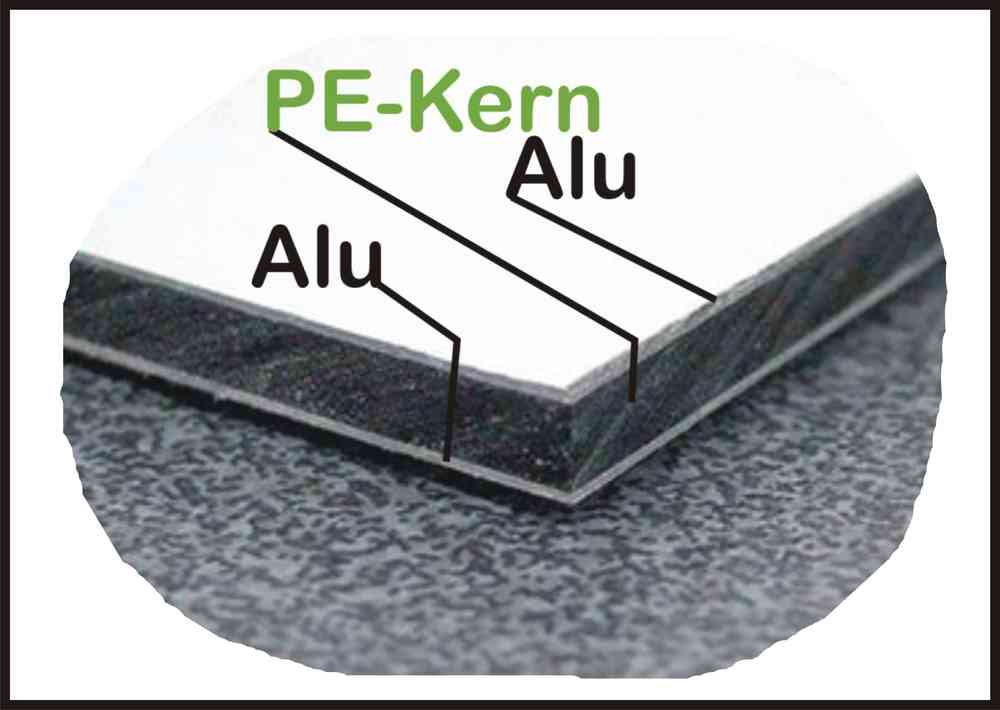
\includegraphics[width=0.5\textwidth]{Dibond_Platten_ml.jpg}
        \caption{Dibond-Platte, Quelle: \cite{Dibond-Platte}}
        \label{fig:Dibond}
    \end{figure}
        
    \paragraph{Digitaler Zwilling}\mbox{}\\
    Moderner Schaltschrankherstellung begegnen im Herstellungsprozess oft große logistische Probleme. Jeder Prozessschritt ist eine Fehlerquelle und wenn Fehler nicht früh erkannt werden, pflanzen sich diese fort. Damit zwischen den Prozessschritten keine Kommunikationsprobleme entstehen setzen viele Hersteller auf das Prinzip des digitalen Zwillings.\\
    Dieser im Grunde ein digitaler Schaltschrank, welcher im ersten Prozessschritt, der Planung, ausgeplant wird und im Herstellungsprozess, sei es der Schrankbau oder die Bestückung, wird einerseits immer derselbe digitale Zwilling aktualisiert und aber auch referenziert. Das heißt alle Prozessschritte beziehen sich auf denselben Plan bzw. digitalen Zwilling (siehe \ref{fig:digilaerZwilling}).\\

    \begin{figure}[H]
        \centering
        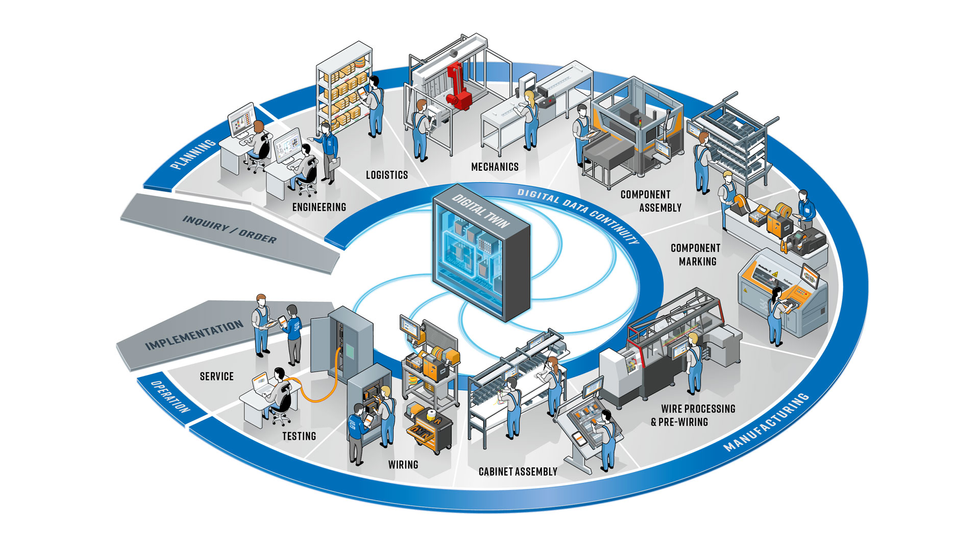
\includegraphics[width=1\textwidth]{Cabinet-Building-Komax-SCB-Component-Printer.png}
        \caption{Digitaler Zwilling, Quelle: \cite{digitaler_zwilling_bild}}
        \label{fig:digilaerZwilling}
    \end{figure}
    
    Es setzt auch ein breites Feld an Firmen auf dieses Prinzip. Firmen wie Weidmüller, Komax, Steinhauer und noch viele mehr haben eine Firmenzusammenarbeit, die ohne einen digitalen Zwilling nicht möglich wäre\cite{smart_cabinet_building}. In diesem Fall werden die jeweiligen Prozessschritte meistens von einer neuen Firma übernommen, in diesem Bündnis ist der digitale Zwilling der Schlüssel zum Erfolg. Man kann dieses Prinzip der Dokumentation bzw. Planung als Industriestandard verstehen.\\
    Um den Prozess der Herstellung des Schaltschrankes möglichst nahe an die Praktiken aus der Industrie anzugleichen, wird auch der Schaltschrank des AFSS mithilfe eines digitalen Zwillings geplant. Dieser wird in Fusion360 gezeichnet und soll den Sollzustand des Schaltschrankes abbilden.\\
    Um den die Konstruktion anzufangen, braucht es eine möglichst ausführliche Ausmessung des bereits bestehenden Serverschrankes. Besonders wichtig sind die Elemente die direkt am Umbau beteiligt sind, wie die Profilschienen (Abstände der Löcher, Abstände der Profilschienen zueinander und detaillierte Abmessungen der Profilschienen selbst.), die Türen und die Lüfter.\\

    \paragraph{Digitaler Zwilling - Schritte}\mbox{}\\  
    Als Erstes muss der Serverschrank, wie bereits erwähnt ausführlich ausgemessen werden. Äußere Höhe, innere Höhe, Äußere Breite, innere Breite und noch Vieles mehr muss richtig gemessen werden. Bei den Messungen werden Messschieber und bei größeren Abständen Maßbänder verwendet. Um die mechanische Konstruktion zu erleichtern, werden alle Daten digital festgehalten.\\
    \begin{wrapfigure}{r}{0.4\textwidth}
        \vspace{-20px}
        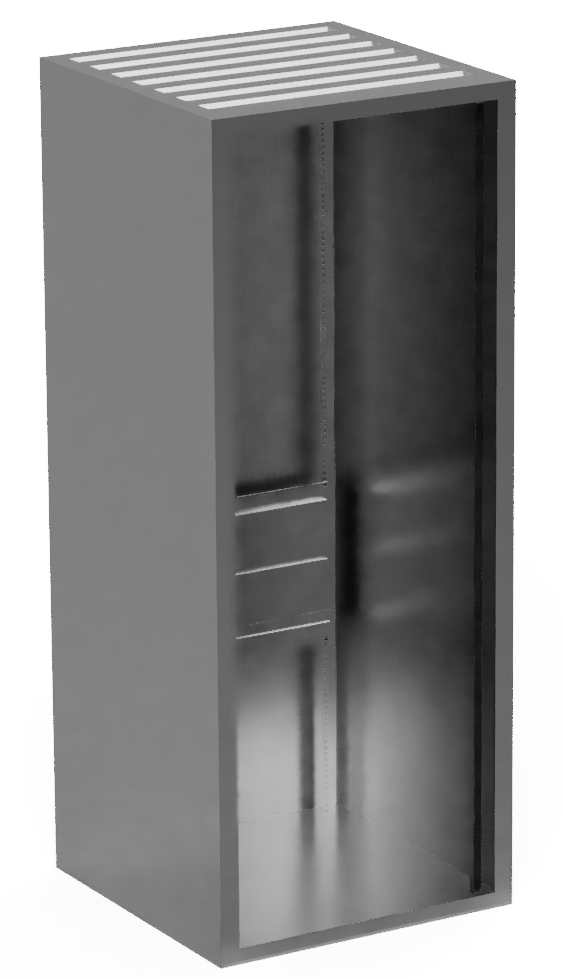
\includegraphics[width=0.39\textwidth]{Prototyp_Serverschrank.PNG}
        \caption{Sommerprototyp eines Serverschrankes}
        \label{fig:Sommerprototyp}
    \end{wrapfigure}
    Während die Messungen des Serverschranks für den finalen digitalen Zwilling wichtig werden, gibt es aber auch noch andere Punkte, beispielsweise bestand lange die Frage, ob das Modulkonzept so möglich sei. Aufgrund dessen und des Umfanges der Diplomarbeit sowie der begrenzten Zeit wird ein erster Entwurf eines Serverschrankes in Fusion360 konstruiert und weiters ein Probemodul gezeichnet. Die Maße dieses digitalen Prototyps sind von einem Standard-Serverschrank aus dem Internet übernommen. Dieser Prototyp hat nicht dieselben Werte wie der richtige Serverschrank, der dem AFSS zur Verfügung steht. Aufgrund der Prototyp-Konstruktion steht fest, dass das Modulkonzept ist so umsetzbar. Weiterführend ist festgestellt, wie man optimierter in Fusion Zeichnen kann. Eine Erkenntnis des Prototyps ist, dass man den Serverschrank nicht als ein großes Element konstruieren sollte, da wenn ein Fehler spät erkannt wird dieser so gut wie nicht mehr zu beheben ist. Wenn die Konstruktion allerdings auf viele verschiedene Elemente aufgeteilt wird, dann ist der Schaden bei einem Fehler begrenzt. 

    Nachdem das Grundprinzip erfolgreich konstruiert wurde, ist der Serverschrank auf Grundlage der echten Maße zu konstruieren. Die gelernten Erkenntnisse werden dabei bestmöglich miteinbezogen.\\
    \begin{wrapfigure}{r}{0.4\textwidth} % 'r' for right, 'l' for left
        \vspace{-20px}
        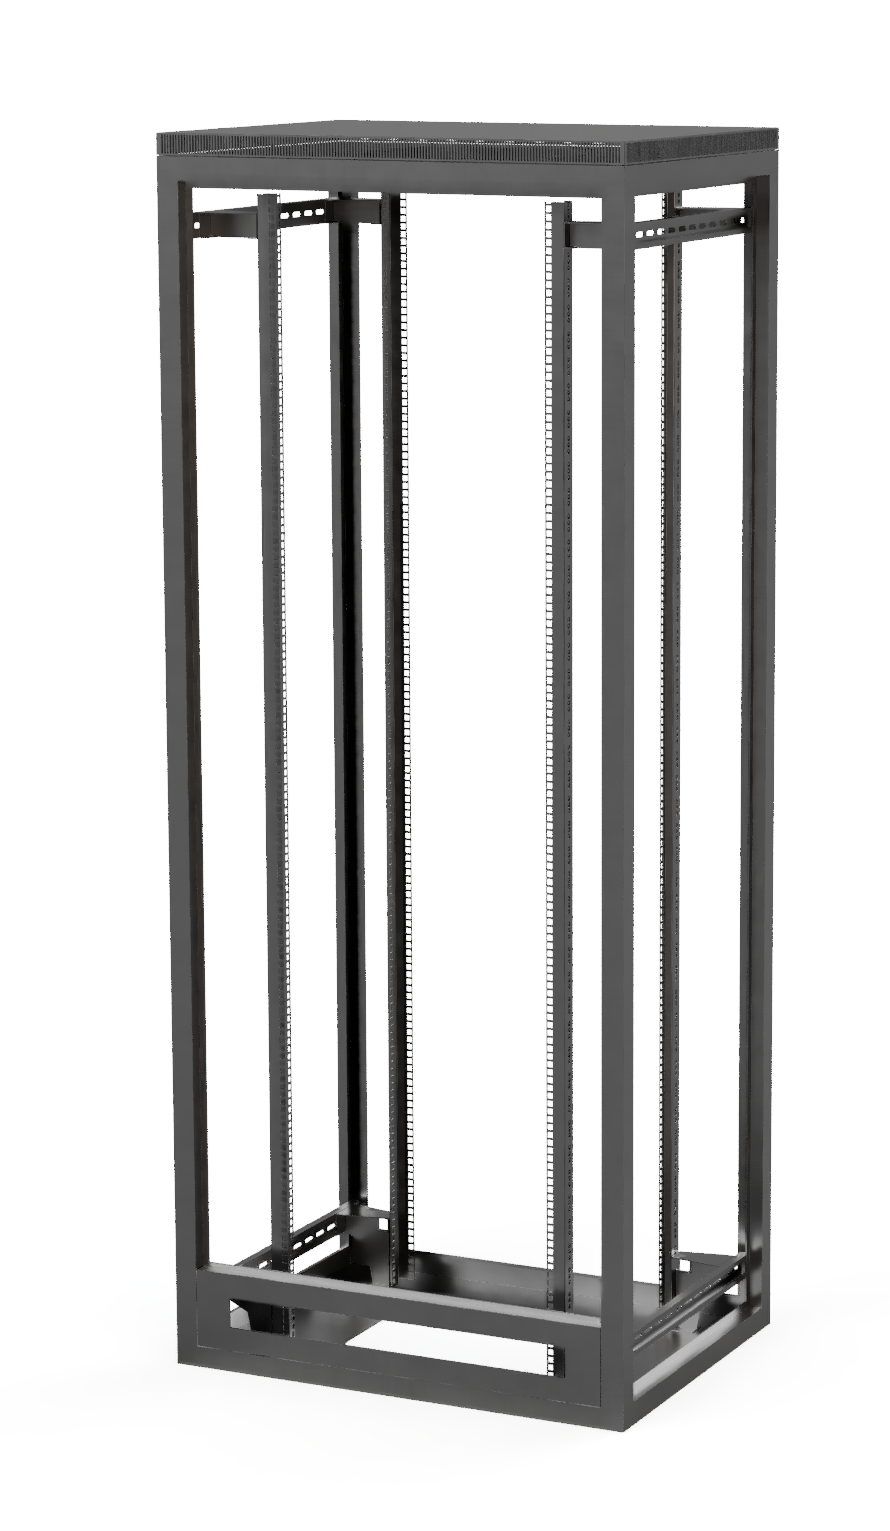
\includegraphics[width=0.4\textwidth]{Schaltschrank_ohne_Module.PNG} % Replace with your image file
        \caption{Serverschrank konstruiert}
        \label{fig:Clean_Serverschrank}
    \end{wrapfigure}
    Mit dem fertig konstruierten Serverschrank, kann dann die Planung der Module beginnen. Dafür wird vorerst ein Konzept erstellt. Durchgedacht wird welche elektrischen Baugruppen wo im Schaltschrank platziert werden sollen. Das Konzept richtet sich einerseits nach der Vorgabe, zusammengehörige Elemente sollen auf dasselbe Modul kommen, und andererseits zusammenhängende Module sollen sich möglichst nahe sein. 
    \paragraph{Modul 1 - Bedienelemente}\mbox{}\\
    Es sollen im Schaltschrank ein Notaus, ein Schlüsselschalter und ein Drehstromschalter verbaut werden. Diese Elemente werden gemeinsam auf einem Modul verbaut, da sie alle Bedienelemente sind.
    \paragraph{Modul 2 bis 3 - Schutzorgane und Versorgungen}\mbox{}\\
    Direkt unter dem Drehstromschalter sollen die Schutzorgane liegen. Da der Leitungsschutzschalter und der Fehlerstromschutzschalter wenig platz benötigen, werden auf dem 2. Modul zusätzlich die zwei Gleichrichter verbaut die auf eine Huttschiene montierbar sind. Damit besteht das 2. Modul aus den Schutzorganen und den Gleichrichtern. Auf die Platte muss damit auch eine durchgängige Huttschine und ein Verdrahtungskanal geplant werden.\\
    Für die reguläre Versorgung des AFSS werden drei normale Gleichrichter benötigt. Der dritte, der Deutronic Gleichrichter, kann nicht auf eine Hutschine montiert werden und hat zudem einen großen Platzbedarf. Dieser wird auf einem eigenen Modul verplant. In den Leerräumen des 3. Moduls werden Hutschinen mit Reihenklemmen verplant. Diese Reihenklemmen sollen für eine übersichtliche Verdrahtung der Versogungsleitungen sorgen.
    \paragraph{Modul 4 - ASI-Elemente}\mbox{}\\
    Konzepttechnisch ist das 4. Modul ein Erweiterungsmodul. Nur eine Ein/Ausgangsbaugruppe von Weidmüller ist auf eine kleine Huttschine verplant gewesen und der restliche Platz sollte freigelassen werden für potentielle Erweiterungen.\\
    Im Entwicklungsprozess ist deutlich geworden, dass die PWM-Signalerzeugung, der Ausgangsbaugruppen, nicht fähig sind ein veränderbares PWM-Signal zu erzeugen. Damit werden diese Elemnte nicht mehr benötigt. Parallel ist verstanden worden, dass es eine getrennte 24V-Versorgung für den ASI-Kreis geben muss. Deswegen ist im ursprünglichen Erweiterungsbereich dieses Modules, ein 24V-ASI-Gleichrichter verplant, der keine Huttschiene benötigt, und anstatt der Weidmüllerkomponenten kommmt eine ET200, an die ein ASI-Master angeschlossen ist. Zudem ist auch ein Verdrahtungskanal nötig.
    \paragraph{Modul 5 - SPS und Sicherungen}\mbox{}\\
    Das 5. Modul beinhaltet die Siemens SPS und die gesammten DC-Sicherungen für die Schrittmotoren. Für die SPS muss eine Siemens-Profilschiene auf die Platte und für die Sicherungen eine durchgängige Huttschiene und einen Verdrahtungskanal.
    \paragraph{Modul 6 - Schrittmotoren}\mbox{}\\
    Für die stärkeren Schrittmotoren werden Treiber verwendet die direkt auf einen Untergund montiert werden müssen. Die vierTreiber werden auf eine eigene Platte montiert. Auch auf diesem Modul ist ein Verdrahtungskanal nötig.
    \paragraph{Modul 7 - Ausgangsmodul}\mbox{}\\
    Am Ausgangsmodul soll einen Verdrahtungskanal haben und eine durchgängige Huttschiene. Auf diese Hutschine kommen Elemente wie die Motorschütz, Relais, die Treiber für die schwächeren Schrittmotoren und eine ausführliche Menge an Reihenklemmen.\\
    \paragraph{Modul 8 - Erdungsmodul}\mbox{}\\
    Etwaige Kabel des AFSS haben einen Schrim der geerdet gehört. Deswegen ist eine Erdungsplatte nötig die aus leitfähigen Aluminium gemacht werden soll. Auf dieser ist eine Ankerschiene geplant. Zudem sollen in dieses Modul vier rechteckige Ausfräsungen gemacht werden, in welche der nichtsteckbare Teil der RJ45-Stecker hineinpasst.\\

    -Module: Ist der Schaltchrank fertig übernommen aus der realität kann man anfangen mit einem Modul. Dabei fällt einem zum Beispiel schon eine sache auf, sowie die Tatsache, dass wenn man die Profilschinen an der selben Position lässt würden sich die Türen nicht schließen lassen. Folge daraus ist, die Profilschinen müssen verschoben werden. Der Aufbau des Serverschranks lässt dies zu.

    -Weitere Module: diese werden dann auch in Fusion360 gezeichnet und dann in den digitalen Zwilling eingefügt. Dabei kann man schön erkennen wie die Module Anneinander gereiht gehören, welche Reihenfolge sinnvoll ist und ob sich die Menge an Elektrischen Einheiten auch ausgeht mit den Modulen. 

    -Dieser soll auch immer die akktuelle version abbilden


\subsection{Realisierung}
\label{sec:Schaltplan}



